% !TeX root = ../Thesis.tex

%*****************************************
\chapter{Related Work}\label{ch:relatedwork}
%*****************************************
\glsresetall % Resets all acronyms to not used

Steganography is often described as both the art and science of hiding information~\cite{bennettLinguisticSteganographySurvey2004}. As its forms are only limited by our creativity, an exhaustive discussion is not possible. Instead, we focus on some selected works. By progressing from simple to more sophisticated approaches, we ultimately answer the question: Why use \glspl{LLM} at all?

\section{Steganography without large language models}
\label{sec:steganographyWithoutLLMs}
As we implement an Android app to perform steganography in chat messages locally on smartphones, hardware resources are our strongest limitation. While \glspl{LLM} are a popular option to perform this kind of steganography~\cite{zieglerNeuralLinguisticSteganography2019}, running them is very resource-intensive. Therefore, we first consider some approaches without \glspl{LLM}.

\subsection{Mimicking}
\label{sec:mimicking}
Spammimic is a demonstration of text-based steganography without \glspl{LLM} from as early as 2001~\cite{spammimicSpammimic2000}. Secret messages are encoded into cover texts that look like spam e-mails. \cref{fig:spammimicSpamEmail} shows an example. This is done using context-free grammars and mimic functions~\cite{waynerMimicFunctions1992,bennettLinguisticSteganographySurvey2004}.

\begin{figure}
    \begin{wide}
        \centering
        \captionsetup{width=\linewidth}
        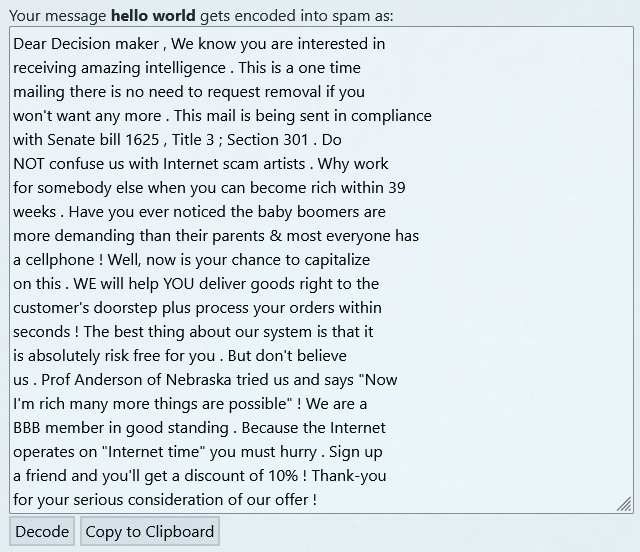
\includegraphics[width=0.5\linewidth]{spammimic_spam_email.png}
        \caption[Spammimic]{Steganography in spam e-mails with Spammimic~\cite{spammimicSpammimic2000}. Only the secret message "hello world" was user input.}
        \label{fig:spammimicSpamEmail}
    \end{wide}
\end{figure}

This approach already fulfills some of the requirements we set ourselves in \cref{ch:introduction}. It generates plausible cover texts for a given topic with minimal computing resources. The topic can be chosen by exchanging the grammar~\cite{spammimicSpammimic2000}. Generating spam e-mails is particularly beneficial as it lowers an attacker's expectation of cover text quality. It allows us to hide our communication amongst other e-mail traffic, obfuscating when a secret communication is happening. We may even send our cover texts to any number of recipients that includes the intended one, to obfuscate who is communicating with whom. Both would increase an attacker's costs significantly~\cite{bennettLinguisticSteganographySurvey2004,petitcolasInformationHidingSurvey1999}.

But there are several drawbacks. Users would have to handle different grammars for different chat conversations. Creating grammars requires expert knowledge. This can't be expected from the average user. In contrast, \glspl{LLM} can be influenced by natural language commands. This can be expected from any layman user. Furthermore, encoding efficiency is low. Any secret message longer than a few words generates cover texts of implausible length, even for a spam e-mail.

\subsection{Substitution}
\label{sec:substitution}
When \gls{SMS} was prevalent, its character limits led users to abbreviate common terms (e.g. "u" for "you"). As shown in ~\cite{shirali-shahrezaTextSteganographySMS2007}, this can be leveraged to perform steganography. We define a dictionary of terms and their abbreviations and let the user write a chat message without any abbreviations. By either substituting terms with their abbreviations or not, we encode 1s and 0s.

This approach again fulfills some of the requirements we set ourselves in \cref{ch:introduction}. It uses minimal computing resources and gives the user great control over cover text quality. Semantically meaningful conversations are guaranteed as terms and their abbreviations are synonymous. A customizable dictionary is already built into the keyboards of most smartphones, so it is easily accessible for the average user.

But there still are several drawbacks. As many terms don't have an abbreviation in practice, encoding efficiency is low. This is aggravated when abbreviations are used for entire sentences instead of individual words (e.g. "ily" instead of "i luv u" for "i love you"). Abbreviations can be undesired for readability or even inappropriate in formal communication. Other substitution approaches (e.g. substituting synonym words) solve these issues only partially.

\subsection{Further considerations}
\label{sec:furtherConsiderations}
In the previous sections of this chapter, we discussed several approaches for text-based steganography without \glspl{LLM}. In particular, we focussed on the extent to which each approach fulfilled our central requirement - creating a believable chat conversation from cover texts. In this section, we take a look at some more text-based steganography approaches, still without involving \glspl{LLM}. But the focus is now on some more refined requirements, stemming from more specific use cases. Lastly, we take a look at an example of what not to do.

\subsubsection{Localization}
\label{sec:localization}
The overall goal of our implementation can be stated as follows: Use text-based steganography in chat messages to protect against attackers. While multiple aspects of this definition can and will be refined over the course of this thesis, we now discuss one aspect that is largely omitted otherwise: Localization. Our standard assumption is that both users and attackers are English-speaking. This may be fine for academic purposes, but in practice a lot of the potential users of our implementation are in countries where English is not an official language. This is especially relevant for protection from political persecution under authoritarian regimes.

An example implementation of location-specific steganography is Nahoft~\cite{united4iranNahoft2021,united4iranU4iadminNahoft2025}. This is an Android app designed to protect people in Iran protesting against their government. It performs text-based steganography by creating cover texts consisting of random Persian words, the official language of Iran. If English was used in this situation, it would only attract unwanted attention from the authorities.

Characteristics specific to languages with non-Latin scripts can be leveraged for steganography. Examples for such languages are Arabic~\cite{shirali-shahrezaNewApproachPersian2006,hamzahLinguisticSteganographyFramework2021,thabitComparativeAnalysisArabic2021}, Chinese~\cite{luoTextSteganographyHigh2017} and Hindi~\cite{allaEvolutionHindiText2009}. The scripts of these languages provide a rich variety of symbols and variations, exceeding what the Latin script has to offer, allowing e.g. multiple equivalent shapes for the same expression~\cite{shirali-shahrezaNewApproachPersian2006,hamzahLinguisticSteganographyFramework2021,thabitComparativeAnalysisArabic2021}. Furthermore, relationships between languages should be considered. Steganography approaches leveraging language-specific characteristics can sometimes be transferred to related languages~\cite{allaEvolutionHindiText2009}.

The challenge of localization can partially be solved with our implementation. As~\cref{ch:design} will explain in detail, one goal of our implementation is that the \gls{LLM} can be swapped out easily. While this doesn't enable us to leverage language specifics like changing character shapes, it enables us to choose a \gls{LLM} that was trained on any natural language desired. If we are able to generate semantically meaningful cover texts in any language, further localization might not be necessary. We could use our implementation in any geo-political conflict, deliberately speaking (or not speaking) the language of the attacker. But verifying this is unfortunately out of scope for this thesis, as the author doesn't speak any languages with non-Latin scripts.

\subsubsection{A negative example}
\label{sec:aNegativeExample}
Lastly, we take a look at an example of what not to do, so we can avoid it in our implementation. We recall that steganography violates Kerckhoffs' principle~\cite{andersonLimitsSteganography1998}, as the security of a steganographic system partially relies on the attacker not knowing the system - or that it is being used in the first place.

An approach for text-based steganography in e-mails is shown in~\cite{malikHighCapacityText2017}. Similar to our implementation, it uses Huffman compression to convert a secret message from string to binary. But instead of generating a cover text with \glspl{LLM}, an edit-based approach is chosen by taking the cover text from user input. Information is encoded by colour coding the cover text, with colours being selected from a user-defined colour table. \cref{fig:colourCoding} shows the example given in~\cite{malikHighCapacityText2017}. As~\cite{malikHighCapacityText2017} proposes, this approach is suitable for personal messages containing congratulations, poems, etc. Users may try to obfuscate the steganography as they have full control over cover text quality and the colour table, e.g. by choosing black, dark grey, light grey and white as colours.

\begin{figure}
    \begin{wide}
        \centering
        \captionsetup{width=\linewidth}
        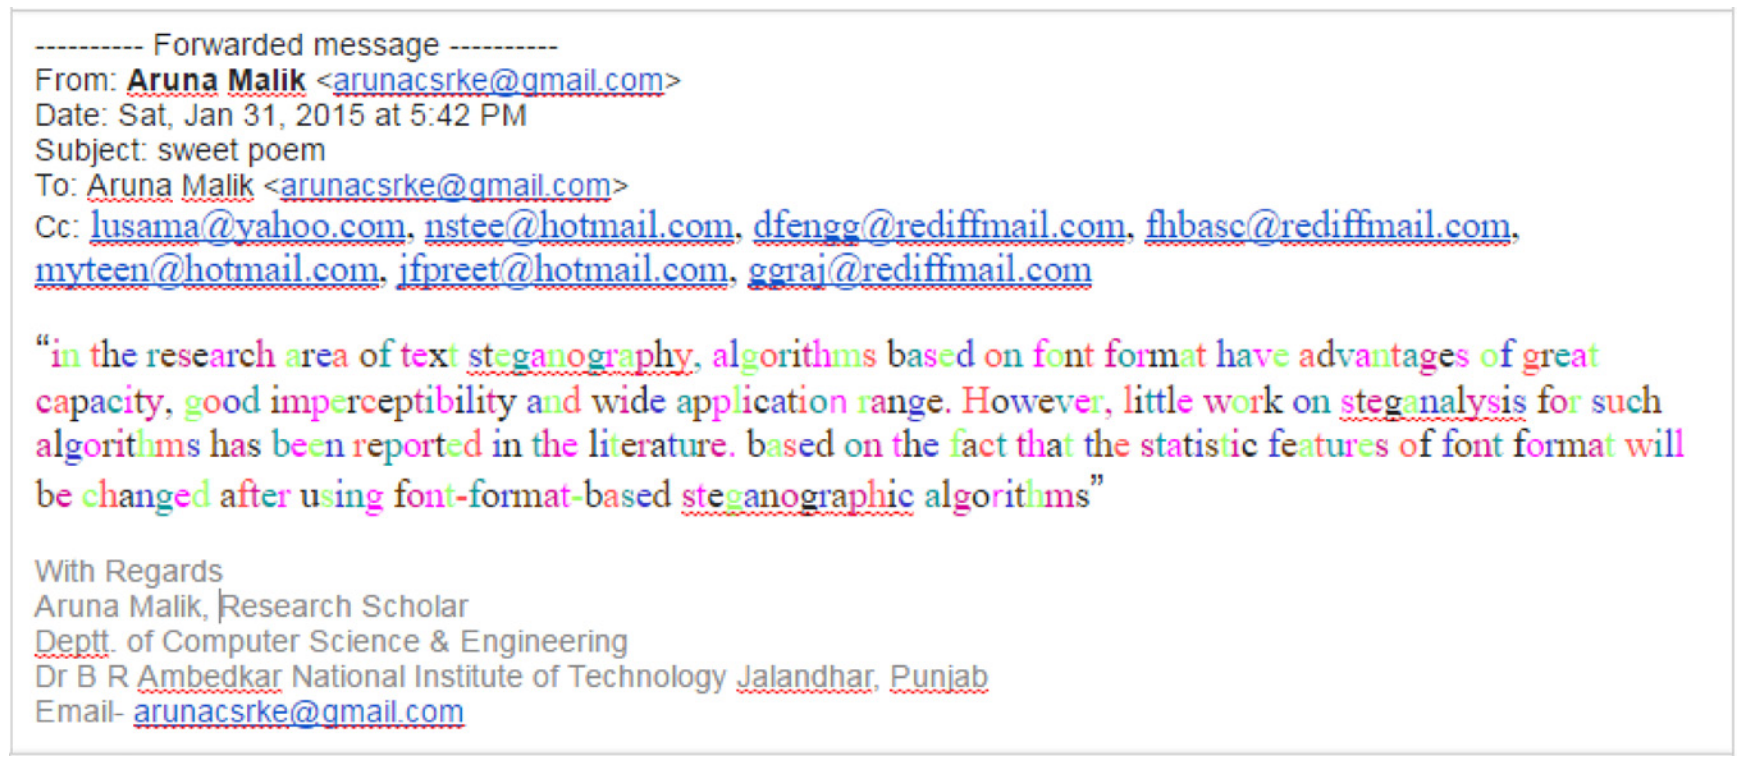
\includegraphics[width=0.75\linewidth]{colour_coding.png}
        \caption[Colour coding]{Steganography via colour coding~\cite{malikHighCapacityText2017}.}
        \label{fig:colourCoding}
    \end{wide}
\end{figure}

However, this doesn't outweigh the disadvantages. The colour table has to be exchanged between sender and receiver, which is difficult as it is not natural language. This approach also is not robust when using non-digital communication channels, as the colour coding is lost if the cover text is spoken during a phone call or printed out in black and white. The proposed use case is very narrow, as an attacker should become suspicious if this is used in any other setting. More generally, the colour coding introduces an unnatural communication pattern that might make it obvious to an attacker that a secret communication is happening. This breaks the additional layer of security that is supposed to be introduced by steganography. We can transfer this to our implementation by avoiding e.g. uncommon use of abbreviations or emojis in the generated chat conversations. Furthermore, we should also avoid introducing unnatural restrictions, e.g. assuming that chat messages are being sent with strictly alternating roles of sender and receiver. \cref{ch:implementation} will show that this is only partially possible in our implementation.

\section{Steganography with large language models}
\label{sec:steganographyWithLLMs}
While steganography approaches without \glspl{LLM} are already able to fulfill some of the requirements we set ourselves in \cref{ch:introduction}, they all suffer from low encoding efficiency. Therefore, we now consider steganography approaches with \glspl{LLM}. First, we restrict ourselves to high-level access via prompting. Then we investigate a low-level solution by manipulating token generation. This finally leads us to the Stegasuras project~\cite{zieglerNeuralLinguisticSteganography2019}, which this thesis is based on.

\subsection{High-level: Prompting}
\label{sec:highLevelPrompting}
With state-of-the-art \glspl{LLM} reaching hundreds of billions of parameters, they are able to perform advanced logic only by being prompted~\cite{hossainLLMProSAnalyzingLarge2025}. As demonstrated in~\cite{steinebachNaturalLanguageSteganography2024} with ChatGPT, we can leverage this to perform steganography. We define two disjoint sets of words, A and B. We prompt the \gls{LLM} to generate a text that contains words from A and B matching a certain pattern (e.g. BABBABABA). We interpret any occurrence of a word from A as 0, any from B as 1.

This approach is attractive because it doesn't require a low-level understanding of \glspl{LLM} to implement it. The topic of cover texts can be controlled via the words in sets A and B, which in turn can be generated via a prompt. Encoding efficiency can be controlled via the number of word sets to choose from. It may also be relatively efficient with computing resources, as the \gls{LLM} is only needed for encoding, not for decoding.

However, this approach conflicts with most of the requirements we set ourselves in \cref{ch:introduction}. As can quickly be tested with tools like LM Studio, small \glspl{LLM} that are feasible to run locally on a smartphone are not able to perform the encoding logic. We would have to rely on a service provider to host a large \gls{LLM} for us. Making core functionality of our app dependent on third parties increases attack surface significantly (see \cref{sec:largeLanguageModels}). Therefore, the simplicity of this approach is not worth it for us.

\subsection{Low-level: Manipulating token generation}
\label{sec:lowLevelManipulatingTokenGeneration}
Many modern frameworks exist to give us low-level access to \glspl{LLM}. As demonstrated in the Stegasuras project with PyTorch and GPT-2~\cite{zieglerNeuralLinguisticSteganography2019,zieglerHarvardnlpNeuralSteganography2025,zieglerStegasuras2025}, this can be leveraged to perform steganography. First, we convert a secret message from string to binary. Then, we encode it into a cover text by letting the \gls{LLM} sample tokens to complete a given context based on the secret message bits. Stegasuras implements UTF-8 conversion and Arithmetic compression for the first step and Arithmetic, Huffman and Bins coding for the second step.

This approach is promising several strengths we haven't seen before. By gaining low-level access to the \gls{LLM}, we can implement a complex encoding logic. This increases encoding efficiency to multiple bits per token and allows us to use small \glspl{LLM} that are feasible to run locally on a smartphone.

However, the Stegasuras implementation also has some shortcomings we can improve upon. Being published in 2019, it is not state-of-the-art anymore. We can expect significant gains in cover text quality by just swapping out the \gls{LLM}~\cite{wuGenerativeTextSteganography2024}. Furthermore, there is an open edge case. Cover text generation ends as soon as all secret message bits are encoded, so the last sentence doesn't get finished~\cite{zieglerStegasuras2025}. Stegasuras offers a partial solution by finishing it with greedy sampling during encoding~\cite{zieglerHarvardnlpNeuralSteganography2025}, but this isn't considered during decoding and therefore adds noise. Stegasuras ignores this in its evaluation by cutting off unfinished last sentences~\cite{zieglerNeuralLinguisticSteganography2019}, thereby corrupting the secret message encoded in them.

Solving this edge case is the first contribution we make. Beyond that, we port the implementation to the state-of-the-art llama.cpp framework~\cite{gerganovGgerganovLlamacpp2024}, which gives us access to a wide range of \glspl{LLM} to scale with available hardware. We implement an Android app to run all of this locally on a smartphone. We extend the functionality by creating chat conversations, allowing users to arbitrarily interleave cover texts and plain texts. We improve cover text quality by including emojis and exposing a system prompt, allowing users to influence \gls{LLM} behaviour on a lower level via a natural language command. This way, we are able to solve the real-world problem of protecting people's privacy against eavesdroppers with steganography.
